\def\firstcircle{(0,0) circle (3cm)}
\def\secondcircle{(0:4cm) circle (3cm)}

\colorlet{circle edge}{blue!50}
\colorlet{circle area}{blue!20}

\tikzset{filled/.style={fill=circle area, draw=circle edge, thick},
    outline/.style={draw=circle edge, thick}}

\begin{center}
% Set A and B
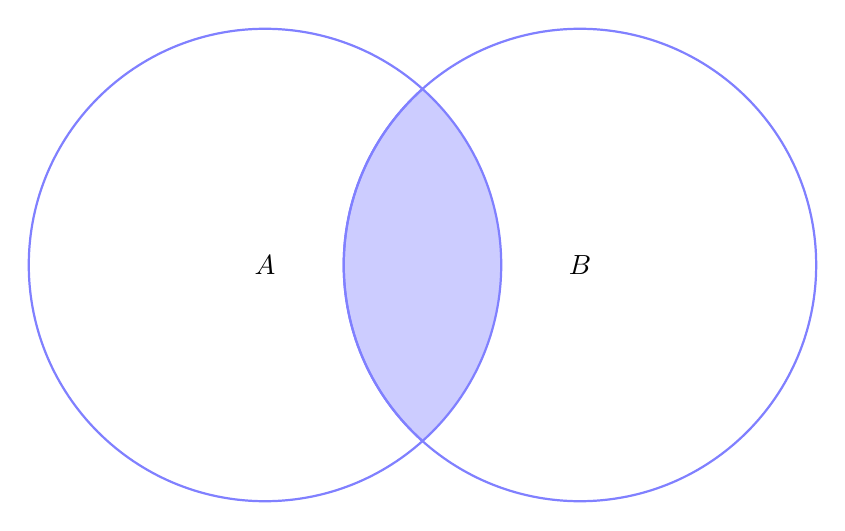
\begin{tikzpicture}
    \begin{scope}
        \clip \firstcircle;
        \fill[filled] \secondcircle;
    \end{scope}
    \draw[outline] \firstcircle node {$A$};
    \draw[outline] \secondcircle node {$B$};
    %\node[anchor=south] at (current bounding box.north) {$A \cap B$};
\end{tikzpicture}
\end{center}

\section{Introduction}
Here we are at the beginning of the mathematics specific content.
Before we get to deep into more complex topics, let us start with what may be considered the most primitive area of mathematics: set theory.
Like most theories, we wouldn't bother having a whole theory for something not punctuated by subtleties.
So we begin as we do with defining what we're talking about; but what is a set?

Naively, we usually say a set is a collection\footnote{I say collection since group is already taken.} of things.
Why is this naive?
You'll see in section~\ref{set:russellsparadox}.

\section{A First Pass At Set Theory}
For out first pass of set theory we will begin with \textbf{Na\"ive Set Theory}, or \textbf{NST}, ignoring future issues for the sake of building a foundational understanding.

\begin{defn}{Naive Set Theory}
  A \textbf{set} is a collection of items.
  It does not matter, for now, what the items are.
\index{element}
  If a particular item, say $a$, is in a set, say $A$, we call $a$ an \textbf{element} of $A$ or we say $a$ is in $A$.
  The boolean operator for establishing membership is $\in$, where $a \in A$ if and only if $a$ is an element of $A$.

  A set is usually denoted as a capitol Roman character.
  Later, we will decorate other symbols which are sets but have additional properties which make them easier to identify.
  To notate the set $A$ with elements $a,b,c$, we write:
  $$
    A = \left\{ a, b, c\right\}.
  $$
\end{defn}

Since any collection can be subdivided into other collections it is useful to make the notion of a \textbf{subset} strict.
To exemplify this, imagine two sets $A$ and $B$.
If each element of $A$ is in $B$ then $A$ is contained within $B$ or, in other words, $A$ is a subset of $B$.
To make this formal, the definition of a subset is as follows:
\begin{defn}{Subset}
  Suppose $A$ and $B$ are two sets.
  For each $a$ if $a$ is in $A$ and it is also in $B$ then $A$ is a \textbf{subset} of $B$.
  Symbolically this case is represented as $A \subset B$.
  Formally, this is represented by:
  $$
    \forall a \left\{ a \in A \implies a \in B \right\}  \Leftrightarrow A \subset B.
  $$
\end{defn}

Having a concept of a subset, we can now define the power set of a set.
\begin{defn}{Power Set}
  Let $A$ be a set.
  The \textbf{power set} of $A$, or $\mathcal{P}(A)$, is the set of all subsets of $A$.
  Formally, this is defined by:
  $$
    \forall x \left\{ x \in \mathcal{P}(A) \iff x \subset A \right\}.
  $$
\end{defn}

If two sets are mutually subsets of each other we say the sets are equivalent.
\begin{defn}{Set Equality}
  Suppose $A$ and $B$ are two sets.
  If $A \subset B$ and $B \subset A$ then $A$ and $B$ are \textbf{equal}, or $A = B$.
\end{defn}
This might at first seems a bit strange as the set $\left\{ a, a, b\right\}$ is the same as the set $\left\{ a, b \right\}$.
In this way, a set with repeated elements or elements in different orders are considered the same.
Later we will discuss different types of objects which do retain these qualities.

We may combine two sets in two distinct ways: we could group everything together, or we could select just the common elements.
The first way, grouping everything together is called the union of two sets as more precisely defined here:
\begin{defn}{Union}
\nomenclature{Union}{The union of two sets is the set of elements in both sets}
  Suppose $A$ and $B$ are two sets.
  The \textbf{union} of $A$ and $B$ is the set of all elements in at least one of the two sets.
  This is symbolically represented as $A \union B$ and is defined by the following sentence:
  $$
  \forall a \left\{ a \in A \union B \iff (a \in A \lor a \in B) \right\}.
  $$
  Using set builder notation, it can be defined as follows:
  $$
    A \union B =  \left\{ a | a \in A \lor a \in B \right\}.
  $$
\end{defn}

For the second way to combine two sets we only collect those elements which are in both sets.
We call this the \textbf{intersection} of two sets.
Formally, this is defined by:
\begin{defn}{Intersection}
\nomenclature{Intersection}{The intersection of two sets is the set of common elements}
  Suppose $A$ and $B$ are two sets.
  The \textbf{intersection} of $A$ and $B$ is the set of all elements at both sets.
  This is symbolically represented as $A \intersection B$ and is defined by the following sentence:
  $$
  \forall a \left\{ a \in A \intersection B \iff (a \in A \land a \in B) \right\}.
  $$
  Using set builder notation, it can be defined as follows:
  $$
    A \intersection B =  \left\{ a | a \in A \land a \in B \right\}.
  $$
\end{defn}


\subsection{Russell's Paradox}
\label{set:russellsparadox}
Russell's Paradox is a simple proof that NST is inconsistent.
The proof is a follows: Imagine you have a set which 

\begin{proof}[Proof of Russell's Paradox]
  To show NST is inconsistent, we suppose the following
  $$
    \exists y \forall x (x \in y \iff P(x))
  $$
  and if $P(x) = x \notin x$, then
  $$
    y \in y \iff y \notin y
  $$
which means \textbf{NST} is inconsistent.
\end{proof}

So what went wrong?
It seems we are unable to make any arbitrary object an element of our set.
To solve this issue multiple theories were created, including Russell's Type Theory and Zermelo Set Theory.

